 \documentclass[a4paper,12pt]{article}
\usepackage[a4paper,top=1.3cm,bottom=2cm,left=1.5cm,right=1.5cm,marginparwidth=0.75cm]{geometry}
\usepackage{setspace}
\usepackage{cmap}					
\usepackage{mathtext} 				
\usepackage[T2A]{fontenc}			
\usepackage[utf8]{inputenc}			
\usepackage[english,russian]{babel}
\usepackage{multirow}
\usepackage{graphicx}
\usepackage{wrapfig}
\usepackage{tabularx}
\usepackage{float}
\usepackage{longtable}
\usepackage{hyperref}
\hypersetup{colorlinks=true,urlcolor=blue}
\usepackage[rgb]{xcolor}
\usepackage{amsmath,amsfonts,amssymb,amsthm,mathtools} 
\usepackage{icomma} 
\mathtoolsset{showonlyrefs=true}
\usepackage{euscript}
\usepackage{mathrsfs}

\DeclareMathOperator{\sgn}{\mathop{sgn}}
\newcommand*{\hm}[1]{#1\nobreak\discretionary{}
	{\hbox{$\mathsurround=0pt #1$}}{}}


\title{\textbf{Изучение колебаний струны (1.4.5)}}
\author{Третьяков Александр}



\begin{document}
	
	\maketitle
	
	\section{Введение}
	
	\textbf{Цели работы:} изучение поперечных стоячих волн на струне; определение собственных частот колебаний струны; исследование зависимости скорости распространения поперечных волн на струне в зависимости от её натяжения.\\
	\textbf{Оборудование:} закрепленная на станине стальная струна, набор грузов,
	электромагнитные датчики, звуковой генератор, двухканальный осциллограф, частотомер.
	
	\section{Теоретические сведения}
	
	Основное свойство струны -- гибкость, является следствием ее большой длины по сравнению с поперечными размерами. Даже струны, изготовленные из жестких материалов, практически не сопротивляются изгибанию, если размер изгибаемого участка значительно больше поперечного размера струны. Данный факт позволяет не учитывать при дальнейшей работе изгибные напряжения.
	
	Горизонтально закрепленная струна провисает под действием поля тяжести, при отсутствии натяжения. Достаточно натянутую струну можно считать прямой, если ее концы закреплены на одном горизонтальном уровне. Учитывая этот факт, в дальнейшем действие силы тяжести учитываться не будет.
	
	Натянутая струна с жестко закрепленными концами удобна для изучения колебаний. Это связанно с тем, что в струне можно непосредственно наблюдать простейшие типы колебаний и волн, измерять их параметры и сравнивать результаты наблюдения с результатами теоретических расчетов.
	
	Движение элементов струны может быть вызвано изменением ее формы или передачей ей импульса. Натяжение струны стремиться вернуть ее в изначальное прямолинейное положение, и это приводит к тому, что возникает движение элементов струны. Возмущения бегут вдоль струны.
	
	Скорость распространения подобного возмущения можно вычислить по формуле \eqref{velocity_of_deformation}.
	
	\begin{equation}
		u = \sqrt{\frac{T}{\rho_l}}
		\label{velocity_of_deformation}
	\end{equation}
	где $F$ -- сила натяжения струны, $\rho_{l}$ -- масса струны на единицу длины.
	
	При заданной частоте $\nu$ длина волны определяется по формуле:
	
	\begin{equation}
		\lambda = \frac{u}{\nu}
	\end{equation}
	
	Частоты собственных колебаний струны определяются формулой:
	
	\begin{equation}
		\nu_{n} = \frac{nu}{2l} = \frac{n}{2l}\sqrt{\frac{T}{\rho_l}}
		\label{frequency_velocity_equation}
	\end{equation}
	где $n$ -- число полуволн, $l$ -- длина струны.
	
	\section{Экспериментальная установка}
	
	\begin{figure}[h!]
		\begin{center}
			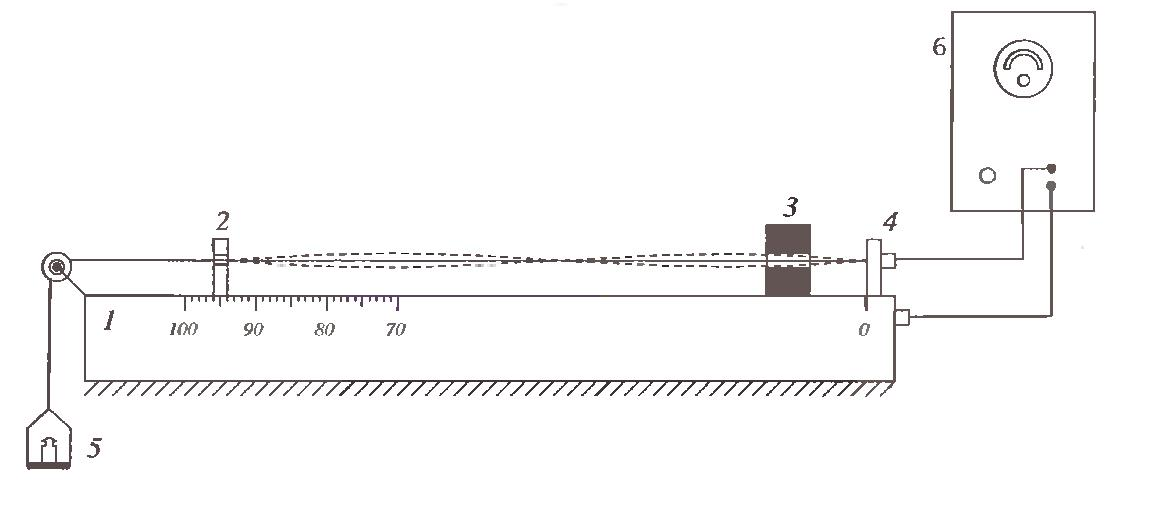
\includegraphics[width = 0.9\textwidth]{1.4.5 ustan}
			\caption{Схема экспериментальной установки}
			\label{facility}
		\end{center}
	\end{figure}
	
	На Рисунке \ref{facility} представлена схема экспериментальной установки. Устроена она следующим образом: на массивной металлической рейке 1 установлены опора 2 и магнит 3, которые можно перемещать вдоль рейки, а также неподвижная опора 4. Один конец струны закреплен в изоляторе опоры 4. От него струна проходит между полюсами магнита и через опору 2, которая дает возможность струне перемещаться в горизонтальной плоскости, неподвижный блок и соединяется с чашкой 5, на которую помещаются грузы. Такое устройство позволяет регулировать натяжение струны.  К концу струны, закрепленному в изоляторе опоры 4, и к массивной металлической рейке 1 подводится переменное напряжение от звукового генератора 6. Движение струны вызывается силой Ампера, действующей на проводник с током со стороны магнитного поля. Частота колебания струны совпадает с частотой вынуждающей силы, т.е с частотой силы Ампера. Так как данная сила зависит от тока в проводнике, то частота колебаний струны будет совпадать с частотой генератора.
	
	В натянутой струне возникнуть колебания, которые сложившись после отражения от опор 2 и 4 создадут стоячую волну, если на длине струны уложится целое число полуволн.
	

\end{document}
